% !TeX root = main.tex
\documentclass[11pt,a4paper]{report}
%%%%%%%%%%%%%%%%%%%%
%   Package setup
%%%%%%%%%%%%%%%%%%%%

\usepackage{array}
\usepackage{tabularx}
\setlength {\marginparwidth }{2cm}
\usepackage{todonotes}
\usepackage{float}
\usepackage{tikz}
\usepackage{hyperref}

%%%%%%%%%%%%%%%%%%%%
%  Document setup
%%%%%%%%%%%%%%%%%%%%

\usepackage[includehead]{geometry}
\usepackage{fancyhdr}

%%%%%%%%%%%%%%%%%%%%
% Custom stuff below
%%%%%%%%%%%%%%%%%%%%

\def\checkmark{\tikz\fill[scale=0.4](0,.35) -- (.25,0) -- (1,.7) -- (.25,.15) -- cycle;} 

\def \principle[#1]{
    \begin{figure}[H]
        \textit{\textbf{Principle -} #1}
    \end{figure}
}
\def \event[#1]{
    \begin{figure}[H]
        \textit{\textbf{Event -} #1}        
    \end{figure}
}
\def \class[#1]{
    \begin{figure}[H]
        \textit{\textbf{Class -} #1}
    \end{figure}
}

\def \ooad[#1]{
    {\tiny \textbf{(OOAD P. #1)}}
}
\author{Mikkel Helsing Andersen}
\title{Object oriented analysis \& design notes}

\begin{document}
    %%%%%%%%%%%%%%%%%%%%
    %  Document setup
    %%%%%%%%%%%%%%%%%%%%
    \pagestyle{fancy}
    \maketitle
    \tableofcontents\label{toc}
    \fancyhead{} % resets header
    \fancyhead[L]{OOAD notes}
    \fancyhead[C]{\textbf{Mikkel Helsing Andersen}}
    \fancyhead[R]{AAU - DAT 3}
    \fancyfoot{} % resets footer
    \fancyfoot[L]{\hyperref[toc]{Table of Contents}}
    \fancyfoot[R]{\thepage}

    %%%%%%%%%%%%%%%%%%%%
    %     Content
    %%%%%%%%%%%%%%%%%%%%
    \chapter{Method}
\section*{Concepets}
\begin{center}
    \begin{tabular}{ l l }
        \hline
        Object & Entity with identity, state and behaviour\\\hline
        Class  & Describes a collection of objects sharing structure, \\ & behavioural patterns and attributes\\\hline
        Problem domain & Part that is administrated, monitored or controlled by a system \\\hline
        Application domain & The organization that administrates the problem domain\\ & Where the user is\\ \hline
        System & A collection components that implements \\ &  modeling requirements, functions and interfaces \\\hline        
        Context & Problem domain and application domain\\\hline
    \end{tabular}
\end{center}
\todo{Describe problem- and application domain better}
\todo{Der er eksempler bag i bogen}

\section*{Problem domain}
Class structure and behaviour

\section*{Application domain}
Usage functions and interfaces

\section*{Method}
Purpose, concepts, principles and results.

\section{Objects and classes}
\subsection*{Objects - \it{Entity with identity, state and behaviour}}
Each object serves as a seperate function. The object could be a customer, where specific people are treated as customers. The object contains that specific customers identity, state and behaviour

\subsection*{Class - \it{Describes a collection of objects sharing structure}}
The class contains multiple objects, meaning a customer class will contain multiple data points. The class also contains multiple different customers and their data points.\\
When describing a class it's important to choose the right granularity. Gravel pit should not be described by the individual grains of sand, instead by the type, whereas a warehouse the individual packages should be described.\\

\subsection*{Analysis - outside the system}
In analysis the object's behaviour is described by its events it performece and experiences that happens in definite points in time. Eg. customers ordering and shipping goods.\\

\subsection*{Design - inside the system}
In design the object's behaviour is described by the operations it can perform and make available to other objects in the system. Eg. add order etc. \\
This allows the update of eg. the customers object state. The design object encapsulates the internal representation of the object state through its operations.\\

\section{Principles}
The 4 principles:
\\\\
\textit{Model the context} -
Useful systems fit the context, so model both application and problem domain during analysis and design.
\\\\
\textit{Emphasize the architecture} -
Understandable architecture makes collaboration between programmers and designers possible. Flexible architecture makes modifications and improvements affordable
\\\\
\textit{Reuse patterns} -
Building on well-established ideas and pretested components
\\\\
\textit{Tailor the method to suit specific project} -
Must be tailored to the specific needs of the analysis and design situation 

\section*{Model}
Model is a representation of the state in the problem domain. How often the model is updated is a design decision\\
Problem domain -> model -> application domain.

    \chapter{System Choice}
Define the system in its context problem domain + application domain.\\
Using the F.A.C.T.O.R system.\\
F: Functionality - System functions that support the AP tasks.
\\\\
A: Application domain
\\\\
C: Condtion
\\\\
T: Technology
\\\\
O: Objects
\\\\
R: Responsibility

\section*{System definition}
\subsection*{Situation}
Describe the situation based on the context of the system. Described in a rich picture.\\
Which is the described by its focus, entities, procceses and structure.

\begin{figure}[h]
    \centering
    \includegraphics*[width=\linewidth]{chapters/system_choice/figure/rich_picture.png}
\end{figure}
\subsection*{Ideas}
Examples - eg. Study preexisting systems.

\subsection*{Context}
    \chapter{Classes \ooad[51]}
To model the problem domain, starting with class activity.

\section{Class Activity}
Abstraction, classification and selection are the primary tasks in the class activity.

\subsection*{Abstraction}
Abstracting the problem domain phenomena by seeing them as objects and events.\\\\

\subsection*{Classification}
Then classifying the objects and events.
\principle[Classify objects in the problem domain]

\textbf{Step 1:} Abstraction and classification should lead to identifying all relevant objects, which should be develop a rich list of potentially relevant classes for the problem-domain model. In a parallel activity, identify and develop a similar list of events.

\subsection*{Selection}
Then selection which classes and events the system will maintain information on. Each class is characterized by a set of specific events.

\textbf{Step 2:} Systematically evaluate the candidates and select relevant classes and events to be included in the problem-domain model. Finally relate events to classes. 

\subsection*{Event table \ooad[52]}
\begin{figure}[H]
    \label{fig:event_table}
    \begin{tabular}{ l | c c c c c }
        \textbf{   Classes} & Customer   & Assistant  & Apprentice & Appointment & Plan      \\
        \textbf{Events}     &            &            &            &             &           \\ \hline
        Reserved            & \checkmark & \checkmark &            & \checkmark  & \checkmark\\
        Cancelled           & \checkmark & \checkmark &            & \checkmark  &           \\
        Treated             & \checkmark &            &            & \checkmark  &           \\
        Employed            &            & \checkmark & \checkmark &             &           \\
        Graduated           &            &            & \checkmark &             &           \\
        Agreed              &            & \checkmark & \checkmark &             & \checkmark\\ \hline
    \end{tabular}
    \caption{Event table for Hair Salon System (P. 52)}
\end{figure}

\section{Classification of Objects and Events \ooad[52]}
\subsection*{Object}
During the problem analysis an object is an abstraction of a phenomena in that problem domain. An object should be indetifiable be an independent entity, which is delimited.
\\
Using events is emphasized by:\\
\principle[Characterize objects through their events]

\subsection*{Event}
Events specify the qualities of problem-domain objects. An event is defined as:\\
\event[An instantaneous incident involving one or more objects]
An event is an abstraction of a problem-domain activity or process that is perfomed or experienced by one or more objects.

\subsection*{Class}
Classes contain objects and event. These are identify all the objects and events to be included in a relevant problem-domain model.
The class concept refers and describse all the objects in a specific class:
\class[A secription of a collection of objects sharing structure, behavioral pattern, and attributes]

Object's structure, behavioral pattern, and attributes are described in general terms by the appopriate class deiniftion. Where all classes are different.

\subsubsection*{Find Classes \ooad[57]}\label{sec:find_classes}
Class selection is the first and most basic for building problem-domain model. It's important to write down all potentially relevant classes, without evaluating them in detail. Do this using own perception, pre-existing decriptions and definitions, including prospective users by interviewing and observing them work. This can be further expanded by using pre-existing system, and using the experience as an advantage. This also include regulations in the are of the operation of the system. This should in a list of class candidates, with easy to understand name, that references in the problem domain.

\subsection*{Event}
\subsubsection*{Find Events \ooad[59]}
Using the same fundamental principle as the \textbf{\hyperref[sec:find_classes]{find classes section}}. 

\subsection*{Evalute Systematically \ooad[62]}
Fundamental evaluation rule: a class or event should be included in the problem-domain model \textit{iff} system functions use information about it. Basic criteria rules:
\begin{itemize}
    \item Is the class or event within the system definition?
    \item Is the class or event relevant for the problem-domain model?
\end{itemize}
Only classes and events within the problem-domain should be selected. These classes and events should refer to phenomena that will be administrated, monitored and controlled by future users in their work. \\\\
Users are usually not part of the problem domain, unless the users are being registered within the system, in eg. the case of restricted access.

\subsubsection*{Evaluation Criteria for Classes \ooad[63]}
As a rule, these questions should be answered when evaluating classes:
\begin{itemize}
    \item Can you identify objects from the classes?
    \item Does the class contain unique information?
    \item Does the class encompass multiple objects?
    \item Does the class have a suitable and manageable number of events?
\end{itemize}
An object should be unambiguously be indetifyalbe from a class. Typically a class will contain multiple objects and should contain an appropriate amount of unique information. Events are realated to classes in order to characterize them. This is expressed through an  \hyperref[fig:event_table]{event table}. Classes can be further specified than their name by descriping their responsibilities, this limits confusion when the system is developed. This is done through plain text and can specify why it differs from other classes.

\subsubsection*{Evaluation Criteria for Events \ooad[65]}
As a rule, these questions should be answered when evaluating events:
\begin{itemize}
    \item Is the event instantaneuou?
    \item Is the event atomic?
    \item Can the event be identified when it happens?
\end{itemize}
It should be defined as instantaneous to make it clear when it happens. If the incident happens over a period a stop and start event can be used. Defining and naming an event determines the granularity of the time model. Each event should be identifiable when it happens.

\subsubsection*{Relating Classes and Event \ooad[66]}
When selecting a class, one also has to define the events that the class objects are involved in. From event to objects should also be defined.
As a rule, these questions should be answered when relating:
\begin{itemize}
    \item Which events is this class involved in?
    \item Which classes are involved in this event?
\end{itemize}
These should be summarized in an \hyperref[fig:event_table]{event table}. Which can also be used to evluate the quality of class and event candidates.
\\\\
{\Large \textbf{Summarized principles can be seen on OOAD P. 66}}
    \chapter{Structure \ooad[71]}\label{chp:structure}
In the structure activity an extension of the problem-domain description to include structural relations between classes. Including relations between objects. The result of the structure activity is a class diagram.

\begin{figure}[H]
    \center
    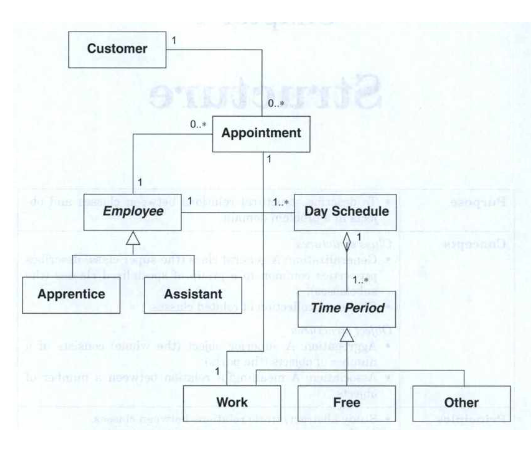
\includegraphics[width=\linewidth*3/4]{chapters/structure/figures/class_diagram.png}
    \caption{Class diagram example \ooad[72]}
    \label{fig:structure_class_diagram}
\end{figure}

\section{Class Structure}
Class structures express static, conceptual relations between classes. They connect classes, and the relationship doesn't change unless the description itself changes.

\subsection*{Generalization}
A general class(super-class) that describes properties common to a group of specialized classes(sub-classes). It's a relation between two or more specialized classes(sub-class) and a general class(super-class). Everything that holds true for the super-class also hold for any sub-classes. Programmingvise its inheritance/extending a super class.\\
This can be tested with "is-a", eg. "doctor is a person" etc.

\subsection*{Cluster}
A collection of related classes. Classes within a structure is usually connected by a generalization class, eg. cars like in \href{fig:structure_cluster_example}{the example below}. Alternatively connected through aggregation structure.
\begin{figure}[H]
    \center
    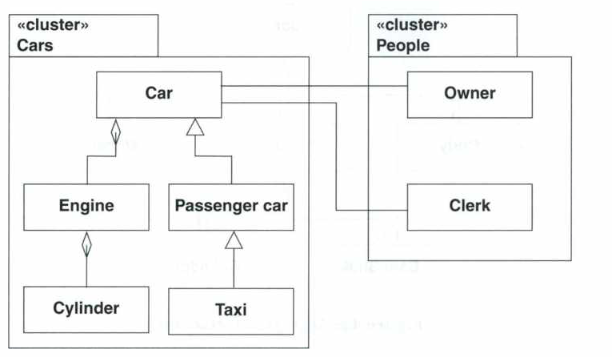
\includegraphics[width=\linewidth*3/4]{chapters/structure/figures/cluster_example.png}
    \caption{Example of clusters and cluster structure \ooad[77]}
    \label{fig:structure_cluster_example}
\end{figure}

\section{Object Structure}
Object structures express dynamic, concrete relations between objects. Theses relationship can change dynamically without changing the underlying description.

\subsection*{Aggregation}
A superior object (the whole) consists of anumber of objects (the part). It's a relation between two or more objects. It expresses that one object is a fundamental and defining part of the other.
\begin{figure}[H]
    \center
    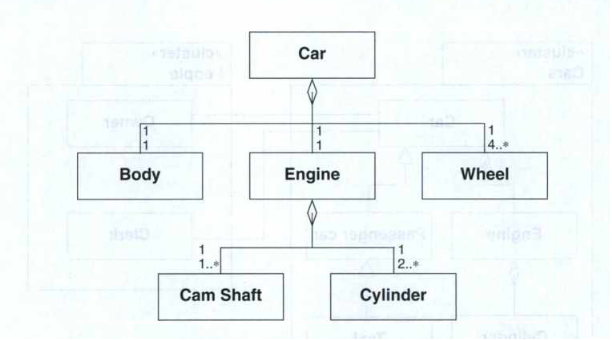
\includegraphics[width=\linewidth*3/4]{chapters/structure/figures/aggregation_structure.png}
    \caption{Aggregation structure example \ooad[78]}
    \label{fig:structure_aggregation_example}
\end{figure}
\subsection*{Association}
A meaningful relation between a number of objects. Objects are not a defining part of an object. The association structure does not define ranking

\section{The Activity}
\begin{figure}[H]
    \center
    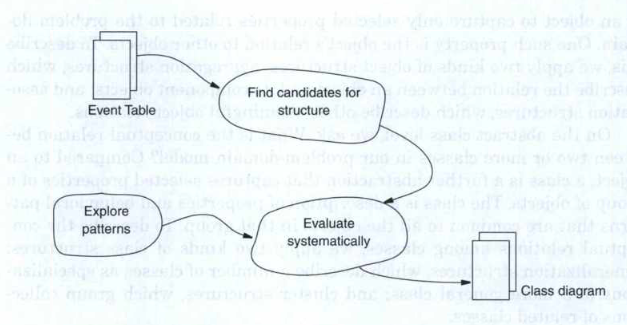
\includegraphics[width=\linewidth*3/4]{chapters/structure/figures/structure_activity.png}
    \caption{Sub-activities involved in the structure activity \ooad[74]}
    \label{fig:structure_structure_activity}
\end{figure}

\section{Finding Structure \ooad[79]}
\subsection*{Finding Candidates}
Similarly to selecting classes and events, it all starts with selecting candidates by brainstorming or other means.

\subsubsection*{Identify Generalization \ooad[80]}
Do this by taking all classes and pair them to see if one is a generalization of the other. \\
Then determine whether it's a relevant relation.\\
Then try to create a relevant specialized or generalized class.

\subsubsection*{Identify Aggregation \ooad[80]}
Find classes with objects that has a decomposition\footnote{Decomposit: The combining of distinct parts or elements to form a whole} object of the other classes. The whole is considered to be superior to its parts, as is reflected in the class diagram by the vertical placement.\\ 
Determine if it's relevant to aggregate the objects of a selected class into a new one. \\
Our third approach is to determine if each class can be decomposed few relevant classes that do not yet exist in the model. Alternatively, consider aggregating the objects of a selected class into a new class.
\\\\
Softer definitions of aggregation:
\begin{itemize}
    \item Whole-part, in which the whole is the sum of the parts, if adding or removing any part, the whole fundamental changes.
    \item Container-Content, in which the whole is a container for the parts, if adding or removing any content, the fundamental properties of the whole doesn't change.
    \item Union-Member, in which the whole is an organized union of members. It doesn't change the union fundamentally by adding or removing a few members. However, there is a lower limit on the number of members, as it is artificial to model a union without members.
\end{itemize}

\subsubsection*{Identify Associations}
See if the remaing class pairs can be meaningfully related. This is done when the relation needs to be administrated, monitored or controlled.

\subsubsection*{Identify Clusters}
Increase class diagrams clarity by organizing conceptually related classes into clusters. A class is not allowed to be in two different clusters.

\section{Explore Patterns \ooad[82]}
\subsection*{The Relation Pattern}
Used when a relation between two objects carry it's own properties.

\subsection*{The Hierarchy Pattern}
When the relation is between multiple objects and are in a hierarchy, where each level organizes into the hierachy. Eg. Student is related to a class which is related to a semester... etc.\\
A variation of this can also have objects related to multiple on a higher level. In this situation the elements are not mutually exclusive.

\subsection*{The Item-Descriptor Pattern}
Where a descriptor class defines specific properties shared by all related objects. This is important in situation where multiple copies are treated as seperate entities, but still share specific properties between them.

\section{Evaluate Systematically \ooad[86]}
\principle[Model only the neccessary structural relations]\\
When evaluating structural relations, it's beneficial to follow certain criteria:
\begin{itemize}
    \item Structures must be  used correctly \ooad[86].\\
    \item Structures must be conceptually true \ooad[87].
    \item Structures must be simple \ooad[88].
\end{itemize}
    \chapter{Behavior \ooad[91]}\label{chapter:behavior}
\begin{figure}[H]
    \begin{tabular}{|l|p{12cm}|}
        \hline
        \textbf{Purpose} & \begin{itemize}
            \item To model the dynamics of a problem domain
        \end{itemize} \\\hline
        \textbf{Concepts} & \begin{itemize}
            \item Event trace: A sequence of events involving a specific object.
            \item Behavioral pattern: A description of possible event traces for all objects in a class.
            \item Attribute: A descriptive property of a class or an event.
        \end{itemize} \\\hline
        \textbf{Principles} & \begin{itemize}
            \item Create behavioral patterns from event traces.
            \item Study common events.
            \item Derive class attributes from behavioral patterns.
        \end{itemize} \\\hline
        \textbf{Result} & \begin{itemize}
            \item A behavioral pattern with attributes for every class in a class diagram.
        \end{itemize} \\\hline
    \end{tabular}
\end{figure}

\section{Behavioral Pattern and Attributes}
In the behavior activity the behavior is described more precisely by adding relative timings to events. Object behavior is defined by an event trace, that exhibits a certain ordering of events.

\subsection*{Event trace \ooad[92]}
\begin{figure}[H]
    \textit{\textbf{Event trace -} A sequence of events involving a specific object}
\end{figure}

An event trace is unique for a single object. It's the precise sequence in a time interval.

\subsection*{Behavioral pattern \ooad[92]}
\begin{figure}[H]
    \textit{\textbf{Behavioral pattern -} A description of possible event traces for all objects in a class.}
\end{figure}
To produce the pattern, examples of event traces for individual objects in a class are used. For problem-domain dynamics, the object collaboration is emphasized; study common events. Common events are used to describe interactions between classes.

\section{Notation for Behavioral Patterns}
\begin{itemize}
    \item (+) Sequence: Events in a set occur one by one.
    \item ($\vert$) Selection: Exactly one out of a set of events occurs.
    \item (*) Iteration: An event occurs zero or more times.
\end{itemize}

\begin{figure}[H]
    \centering
    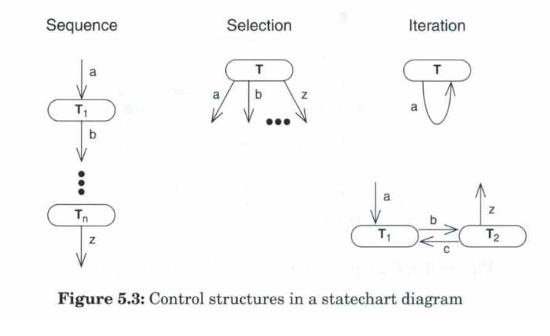
\includegraphics[width=\linewidth]{chapters/behavior/figures/statechart.png}
\end{figure}

\begin{figure}[H]
    \centering
    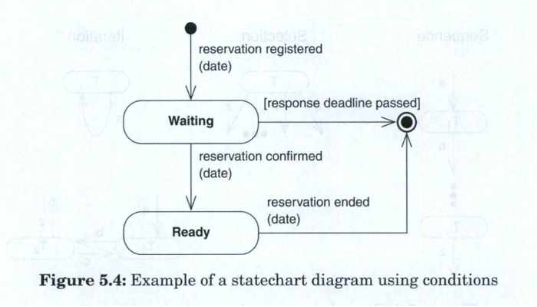
\includegraphics[width=\linewidth]{chapters/behavior/figures/condtion_statechart.png}
\end{figure}

\section{Describe Behavioral Patterns \ooad[98]}
In the class activity the connection between classes and events was created in an event table. These unordered events can then be ordered by identifying the first and last events in an objects life.
\begin{itemize}
    \item Which events cause the creation of a problem-domain object? These events are grouped as selections that can cause the birth of an object.
    \item Which events cause the disappearance of a problem-domain object? These events are grouped as selections that can cause the death of an object.
\end{itemize}
An object is birthed when the first event is triggered, and is dead when the last occurs. This does however not mean it ceases to exists, only events cannot occur on it any more.
\\\\
Generally ensure that the problem-domain model includes both structured and unstructured forms of behavioral patterns.

\subsection*{Unstructured}
The unstructured form contains a collection of intermediate events in a combination of selction and iteration. Meaning events can occur an arbitrary amount of times in an arbitrary order.

\subsection*{Structured}
Characterized by an overall sequence, that includes all major events between birth and death. Physical objects and documents are often described this way.
\\\\
When describing behavioral patterns using event traces, ask these questions:
\begin{itemize}
    \item Is the overall form structured or unstructured?
    \item Which events occur together in a sequence?
    \item Are there any alternative events?
    \item Can a given event occur more than once?
\end{itemize}

\subsection*{Sufficient, but Simple \ooad[100]}
Some times conflicting goals:
\begin{itemize}
    \item The behavioral pattern should be sufficiently precise to describe all legal, and thus all illegal, event traces.
    \item The behavioral pattern should provide an overview and thus be as simple as possible.
\end{itemize}
The first goal is to capture all allowable event traces sufficiently, by describing typical behavior.\\
The second goal is to make simple descriptions.
\subsection*{Inheritance of Behavioral Patterns \ooad[102]}
Specialized classes will inherited its super classes behavior, and usually build more sub-patterns on top. Inheritance means it inherites all behavior and their timings.

\section{Explore Patterns \ooad[104]}
Three different models.

\subsection*{The Stepwise Relation Pattern \ooad[104]}
Stepwise relation pattern is used when certain objects are related to the elements of a hierarchy in a stepwise of sequential manner.
\begin{figure}[H]
    \centering
    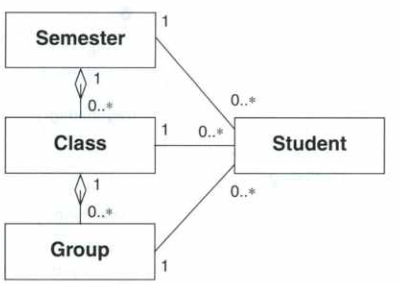
\includegraphics[width=\linewidth/2]{chapters/behavior/figures/stepwise_relation.png}
\end{figure}
\subsection*{The Stepwise Role Pattern \ooad[104]}
\begin{figure}[H]
    \centering
    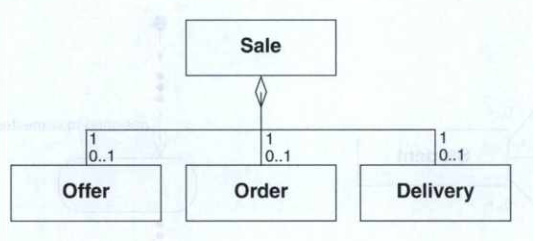
\includegraphics[width=\linewidth/2]{chapters/behavior/figures/stepwise_role.png}
\end{figure}

\subsection*{The Composite Pattern \ooad[107]}
The composite pattern offers a way to describe the creation and destruction of a hierarchy using a detailed structure that is unknown at model-development time. 
\begin{figure}[H]
    \centering
    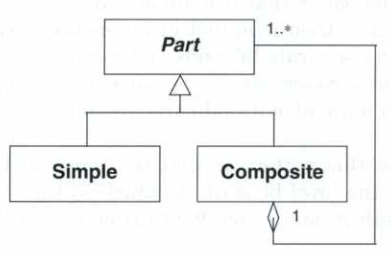
\includegraphics[width=\linewidth/2]{chapters/behavior/figures/composite_pattern.png}
\end{figure}

\section{Consider Structure}
\subsection*{Aggregation and Association\ooad[108]}
\begin{itemize}
    \item If two or more objects have common events, consider adding an aggregation or association structure between them.
    \item If two classes are related by an aggregation or association structure, at least one common event should be considered.
\end{itemize}

\subsection*{Generalization \ooad[109]}
\begin{itemize}
    \item If the same event is tied to two classes, consider whether one class is a generalization of the other.
    \item If two classes have many events with the same name, consider whether they are different specializations of a third class.
\end{itemize}
\end{document}